\newcommand{\coursepath}{/teaching/2021/ConcDisSys}
\newcommand{\courseurl}{\url{https://www.cst.cam.ac.uk\coursepath}}
\newcommand{\thisyear}{2020/21}

\fancypagestyle{plain}{%
  \renewcommand{\headrulewidth}{0pt}%
  \fancyhf{}%
  \fancyfoot[C]{%
      \raisebox{-0.15cm}{
\includegraphics[height=0.5cm]{images/creative-commons.png}}\hspace{5pt}
      This work is published under a \href{https://creativecommons.org/licenses/by-sa/4.0/}{Creative Commons BY-SA license}.%
  }%
}

\begin{document}
\title{Distributed Systems}
\subtitle{University of Cambridge\\Computer Science Tripos, Part IB\\Michaelmas term \thisyear\\\courseurl}
        
\author{Dr.\ Martin Kleppmann\\mk428@cst.cam.ac.uk}
\date{}
\maketitle

\def\sectionautorefname{Section}%
\def\subsectionautorefname{Section}%
\def\subsubsectionautorefname{Section}%

\section{Introduction}

\begin{frame}
    \label{s:title}
    \begin{center}
        \textbf{\huge{\color{darkblue}{Distributed Systems}}} \\[2em]
        The second half of \emph{Concurrent and Distributed Systems}\\[0.5em]
        \url{https://www.cl.cam.ac.uk/teaching/current/ConcDisSys}\\[2em]
        Dr.\ Martin Kleppmann (mk428@cam) \\[0.5em]
        University of Cambridge \\[0.5em]
        Computer Science Tripos, Part IB \\[2em]
    \end{center}
    \begin{columns}[totalwidth=9cm]
        \begin{column}{4cm}
            \hfill
\includegraphics[height=0.5cm]{images/creative-commons.png}\hspace{5pt}
        \end{column}
        \begin{column}{5cm}\scriptsize
            This work is published under a\\\href{https://creativecommons.org/licenses/by-sa/4.0/}{Creative Commons BY-SA license}.
        \end{column}
    \end{columns}
\end{frame}

This 8-lecture course on distributed systems forms the second half of \emph{Concurrent and Distributed Systems}.
While the first half focussed on concurrency among multiple processes or threads running on the same computer, this second half takes things further by examining systems consisting of multiple communicating computers.

Concurrency on a single computer is also known as \emph{shared-memory concurrency}, since multiple threads running in the same process have access to the same address space.
Thus, data can easily be passed from one thread to another: a variable or pointer that is valid for one thread is also valid for another.

This situation changes when we move to distributed systems.
We still have concurrency in a distributed system, since different computers can execute programs in parallel.
However, we don't typically have shared memory, since each computer in a distributed system runs its own operating system with its own address space, using the memory built into that computer.
Different computers can only communicate by sending each other messages over a network.

(Limited forms of distributed shared memory exist in some supercomputers and research systems, and there are technologies like \emph{remote direct memory access} (RDMA) that allow computers to access each others' memory over a network.
Also, databases can in some sense be regarded as shared memory, but with a different data model compared to byte-addressable memory.
However, broadly speaking, most practical distributed systems are based on message-passing.)

Each of the computers in a distributed system is called a \emph{node}.
Here, ``computer'' is interpreted quite broadly: nodes might be desktop computers, servers in datacenters, mobile devices, internet-connected cars, industrial control systems, sensors, or many other types of device.
In this course we don't distinguish them: a node can be any type of communicating computing device.

\begin{frame}
    \label{s:dist-sys-definition}
    \frametitle{A distributed system is\dots}
    \begin{itemize}
        \item<1-> \emph{``{\dots}a system in which the failure of a computer you didn't even know existed can render your own computer unusable.''} --- Leslie Lamport\\[1em]
        \item<2> {\dots}multiple computers communicating via a network\dots
        \item<2> {\dots}trying to achieve some task together
        \item<2> Consists of ``nodes'' (computer, phone, car, robot, \dots)
    \end{itemize}
    \hfill\includegraphics<1>[height=4cm]{images/lamport.jpg}
\end{frame}
\inlineslide{s:dist-sys-definition}\label{l:dist-sys-definition}
% reference for Lamport quote: https://www.microsoft.com/en-us/research/publication/distribution/
% License for photo: https://commons.wikimedia.org/wiki/File:Leslie_Lamport.jpg

\subsection{About this course}

These notes and the lecture recordings should be self-contained, but if you would like to read up on further detail, there are several suggested textbooks:
\begin{itemize}
    \item Maarten van Steen and Andrew S.\ Tanenbaum. \emph{Distributed Systems}. ISBN 978-1543057386.
        Free download from \url{https://www.distributed-systems.net/index.php/books/ds3/} (third edition, 2017).

        This book gives a broad overview over a large range of distributed systems topics, with lots of examples from practical systems.

    \item Christian Cachin, Rachid Guerraoui, and Luís Rodrigues.
        \emph{Introduction to Reliable and Secure Distributed Programming}.
        Second edition, Springer, 2011. ISBN 978-3-642-15259-7.

        Ebook download for Cambridge users: \url{https://link.springer.com/book/10.1007/978-3-642-15260-3} then click Log in $\rightarrow$ via Shibboleth $\rightarrow$ type \emph{University of Cambridge} $\rightarrow$ log in with Raven.

        This book is more advanced, going into depth on several important distributed algorithms, and proving their correctness.
        Recommended if you want to explore the theory in greater depth than this course covers.

    \item Martin Kleppmann. \emph{Designing Data-Intensive Applications}, O'Reilly, 2017. ISBN 978-1449373320.

        This book goes more in the direction of databases, but also covers a number of distributed systems topics.
        It is designed for software engineers in industry working with distributed databases.

    \item Jean Bacon and Tim Harris. \emph{Operating Systems: Concurrent and Distributed Software Design}.
        Addison-Wesley, 2003. ISBN 978-0321117892.

        This book provides a link to the \emph{concurrent systems} half of the course, and to operating systems topics.
\end{itemize}

Where appropriate, these lecture notes also contain references to research papers and other useful background reading (these are given in square brackets, and the details appear at the end of this document).
However, only material covered in the lecture notes and videos is examinable.

\begin{frame}
    \label{s:reading}
    \frametitle{Recommended reading}
    \begin{itemize}
        \item van Steen \& Tanenbaum.\\ ``\textbf{Distributed Systems}''\\(any ed), free ebook available
        \item Cachin, Guerraoui \& Rodrigues. \\ ``\textbf{Introduction to Reliable and Secure Distributed Programming}'' (2nd ed), Springer 2011
        \item Kleppmann.\\ ``\textbf{Designing Data-Intensive Applications}'',\\O’Reilly 2017
        \item Bacon \& Harris.\\ ``\textbf{Operating Systems: Concurrent and Distributed Software Design}'', Addison-Wesley 2003
    \end{itemize}
\end{frame}
\inlineslide{s:reading}

The syllabus, slides, and lecture notes for this course have been substantially revised for 2020/21.
This means that new mistakes may have crept in.
If you notice anything wrong, or if anything is unclear, please let me know by email (\url{mk428@cst.cam.ac.uk})!

As for other courses, past exam questions are available at \url{https://www.cl.cam.ac.uk/teaching/exams/pastpapers/t-ConcurrentandDistributedSystems.html}.
Because of syllabus changes, some of the past exam questions are no longer applicable.
TODO: details on which questions are obsolete.

These notes also contain exercises, which are suggested material for discussion in supervisions.
Solution notes for supervisors are available from the course web page.

This course is related to several other courses in the tripos, as shown on \autoref{l:other-courses}.

\begin{frame}
    \label{s:other-courses}
    \frametitle{Relationships with other courses}
    \begin{itemize}
        \item \textbf{Concurrent Systems} -- Part IB\\
            (every distributed system is also concurrent)
        \item \textbf{Operating Systems} -- Part IA\\
            (inter-process communication, scheduling)
        \item \textbf{Databases} -- Part IA\\
            (many modern databases are distributed)
        \item \textbf{Computer Networking} -- Part IB Lent term\\
            (distributed systems involve network communication)
        \item \textbf{Further Java} -- Part IB Michaelmas\\
            (distributed programming practical exercises)
        \item \textbf{Security} -- Part IB Easter term\\
            (network protocols with encryption \& authentication)
        \item \textbf{Cloud Computing} -- Part II\\
            (distributed systems for processing large amounts of data)
    \end{itemize}
\end{frame}
\inlineslide{s:other-courses}\label{l:other-courses}


\subsection{Pros and cons of distributed systems}

There are a number of reasons for creating distributed systems.
Some applications are \emph{instrinsically distributed}: if you want to send a message from your phone to your friend's phone, that operation inevitably requires those phones to communicate via some kind of network.

Some distributed systems do things that in principle a single computer could do, but they do it \emph{more reliably}.
A single computer can fail and might need to be rebooted from time to time, but if you are using multiple nodes, then one node can continue serving users while another node is rebooting.
Thus, a distributed system has the potential to be more reliable than a single computer, at least if it is well-designed (somewhat contradicting Lamport's quote on \autoref{l:dist-sys-definition})!

Another reason for distribution is for better \emph{performance}: if a service has users all over the world, and they all have to access a single node, then either the users in the UK or the users in New Zealand are going to find it slow (or both).
By placing nodes in multiple locations around the world, we can get around the slowness of the speed of light by routing each user to a nearby node.

Finally, some large-scale data processing or computing tasks are simply \emph{too big} to perform on a single computer, or would be intolerably slow.
For example, the Large Hadron Collider at CERN is supported by a worldwide computing infrastructure with 1 million CPU cores for data analysis, and 1 exabyte ($10^{18}$ bytes) of storage! See \url{https://wlcg-public.web.cern.ch/}.

\begin{frame}
    \label{s:why-distribute}
    \frametitle{Why make a system distributed?}
    \begin{itemize}\pause
        \item \textbf{It's inherently distributed:}\\e.g. sending a message from your mobile phone to your friend's phone\pause
        \item \textbf{For better reliability:}\\even if one node fails, the system as a whole keeps functioning\pause
        \item \textbf{For better performance:}\\get data from a nearby node rather than one halfway round the world\pause
        \item \textbf{To solve bigger problems:}\\e.g. huge amounts of data, can't fit on one machine
    \end{itemize}
\end{frame}
\inlineslide{s:why-distribute}

However, there are also downsides to distributed systems, because things can go wrong, and the system needs to deal with such faults.
The network may fail, leaving the nodes unable to communicate.

\begin{frame}
    \label{s:no-internet}
    
\includegraphics[height=\paperheight]{images/no-internet.png}
\end{frame}
\inlineslide{s:no-internet}

Another thing that can go wrong is that a node may crash, or run much slower than usual, or misbehave in some other way (perhaps due to a software bug or a hardware failure).
If we want one node to take over when another node crashes, we need to detect that a crash has happened; as we shall see, even that is not straightforward.
Network failures and node failures can happen at any moment, without warning.

In a single computer, if one component fails (e.g.\ one of the RAM modules develops a fault), we normally don't expect the computer to continue working nevertheless: it will probably just crash.
Software does not need to be written in a way that explicitly deals with faulty RAM.
However, in a distributed system we often \emph{do} want to tolerate some parts of the system being broken, and for the rest to continue working.
For example, if one node has crashed (a \emph{partial failure}), the remaining nodes may still be able to continue providing the service.

If one component of a system stops working, we call that a \emph{fault}, and many distributed systems strive to provide \emph{fault tolerance}: that is, the system as a whole continues functioning despite the fault.
Dealing with faults is what makes distributed computing fundamentally different, and often harder, compared to programming a single computer.
Some distributed system engineers believe that if you can solve a problem on a single computer, it is basically easy!
Though, in fairness to our colleagues in other areas of computer science, this is probably not true.

\begin{frame}
    \label{s:why-not}
    \frametitle{Why NOT make a system distributed?}
    The trouble with distributed systems:
    \begin{itemize}
        \item Communication may fail (and we might not even know it has failed).
        \item Processes may crash (and we might not know).
        \item All of this may happen nondeterministically.
    \end{itemize}\vspace{1em}\pause
    \textbf{Fault tolerance}: we want the system as a whole to continue working, even when some parts are faulty.\\[1em]
    This is hard.\\[1em]
    Writing a program to run on a single computer is comparatively easy?!
\end{frame}
\inlineslide{s:why-not}


\subsection{Distributed systems and computer networking}

When studying distributed systems, we usually work with a high-level abstraction of the hardware.

\begin{frame}
    \label{s:networking}
    \frametitle{Distributed Systems and Computer Networking}
    We use a simple abstraction of communication:
    \begin{center}
        \begin{tikzpicture}
            \node [circle,fill=red!10,draw] (i) at (0,0) {node $i$};
            \node [circle,fill=red!10,draw] (j) at (6,0) {node $j$};
            \draw [bigarrow] (i) -- node [above] {message $m$} (j);
        \end{tikzpicture}
    \end{center}\pause

    Reality is much more complex:
    \begin{itemize}
        \item \textbf{Various network operators:}\\ eduroam, home DSL, cellular data, coffee shop wifi, submarine cable, satellite\dots\\[1em]
        \item \textbf{Physical communication:}\\ electric current, radio waves, laser, hard drives in a van\dots
    \end{itemize}
\end{frame}
\inlineslide{s:networking}

In this course, we just assume that there is some way for one node to send a message to another node.
We don't particularly care how that message is physically represented or encoded~-- the network protocols, informally known as the \emph{bytes on the wire}~-- because the basic principle of sending and receiving messages remains the same, even as particular networking technologies come and go.
The ``wire'' may actually be radio waves, lasers, a USB thumb drive in someone's pocket, or even hard drives in a van.

\begin{frame}[plain]
    \label{s:snowball}
    \frametitle{Hard drives in a van?!}
    \begin{center}
        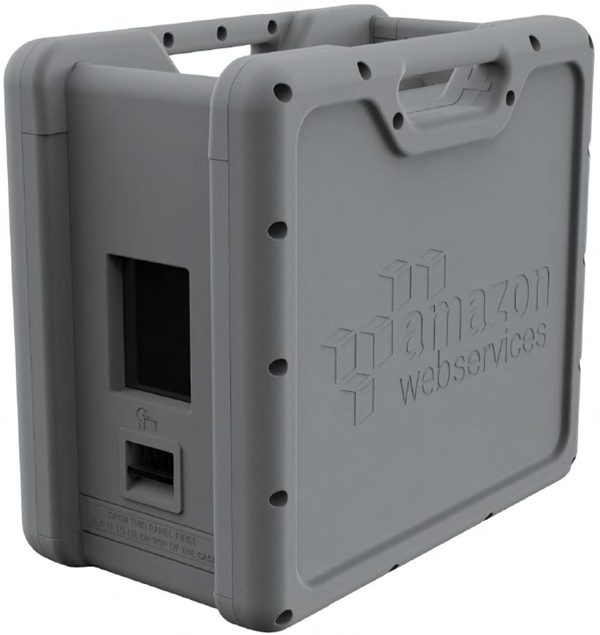
\includegraphics[height=5cm]{images/aws-snowball.png}\\[0.5em]
        \scriptsize{\url{https://docs.aws.amazon.com/snowball/latest/ug/using-device.html}}\\[2em]
        High latency, high bandwidth!
    \end{center}
\end{frame}
\inlineslide{s:snowball}

Indeed, if you want to send a very large message (think tens of terabytes), it would be slow to send that data over the Internet, and it is in fact faster to write that data to a bunch of hard drives, load them into a van, and to drive them to their destination.
But from a distributed systems point of view, the method of delivering the message is not important: we only see an abstract communication channel with a certain \emph{latency} (delay from the time a message is sent until it is received) and \emph{bandwidth} (the volume of data that can be transferred per unit time).

The Computer Networking course in Lent term focusses on the network protocols that enable messages to get to their destination.
The study of distributed systems builds upon that facility, and instead focusses on how several nodes should coordinate in order to achieve some shared task.
The design of distributed algorithms is about deciding what messages to send, and how to process the messages when they are received.

\begin{frame}
    \label{s:latency-bandwidth}
    \frametitle{Latency and bandwidth}
    \textbf{Latency}: time until message arrives
    \begin{itemize}
        \item In the same building/datacenter: $\approx 1$ ms
        \item One continent to another: $\approx 100$ ms
        \item Hard drives in a van: $\approx 1$ day\\[2em]
    \end{itemize}\pause
    \textbf{Bandwidth}: data volume per unit time
    \begin{itemize}
        \item 3G cellular data: $\approx 1$ Mbit/s
        \item Home broadband: $\approx 10$ Mbit/s
        \item Hard drives in a van: 50~TB/box $\approx 1$ Gbit/s\\[1em]
    \end{itemize}
    (Very rough numbers, vary hugely in practice!)
\end{frame}
\inlineslide{s:latency-bandwidth}

\subsection{Example: the web, a client-server distributed system}\label{sec:web}

The web is an example of a distributed system that you use every day.

\begin{frame}[plain]
    \label{s:website}
    \begin{tikzpicture}[remember picture,overlay]
        \node at (current page.center) {
\includegraphics[height=\paperheight]{images/website.png}};
    \end{tikzpicture}
\end{frame}
\inlineslide{s:website}

\begin{frame}
    \label{s:client-server}
    \frametitle{Client-server example: the web}
    Time flows from top to bottom.
    \begin{center}
        \begin{tikzpicture}
            \node [rectangle,fill=red!10,draw] (client) at (0,4) {client};
            \node [rectangle,fill=red!10,draw] (server) at (8,4) {server www.cst.cam.ac.uk};
            \draw (client) -- (0,0);
            \draw (server) -- (8,0);
            \draw<2-> [bigarrow] (0,3) -- node [above,sloped] {GET \coursepath} (8,2);
            \draw<3> [bigarrow] (8,1.5) -- node [above,sloped] {\texttt{<!DOCTYPE html><html>...}} (0,0.5);
        \end{tikzpicture}
    \end{center}
\end{frame}
\inlineslide{s:client-server}

In the web there are two main types of nodes: \emph{servers} host websites, and \emph{clients} (web browsers) display them.
When you load a web page, your web browser sends a \emph{HTTP request} message to the appropriate server.
On receiving that request, the web server sends a \emph{response} message containing the page contents to the client that requested it.
These messages are normally invisible, but we can capture and visualise the network traffic with a tool such as Charles (\url{https://www.charlesproxy.com/}), shown on \autoref{l:http-capture}.

\begin{frame}[plain]
    \label{s:http-capture}
    \begin{tikzpicture}
        \node at (0,0) {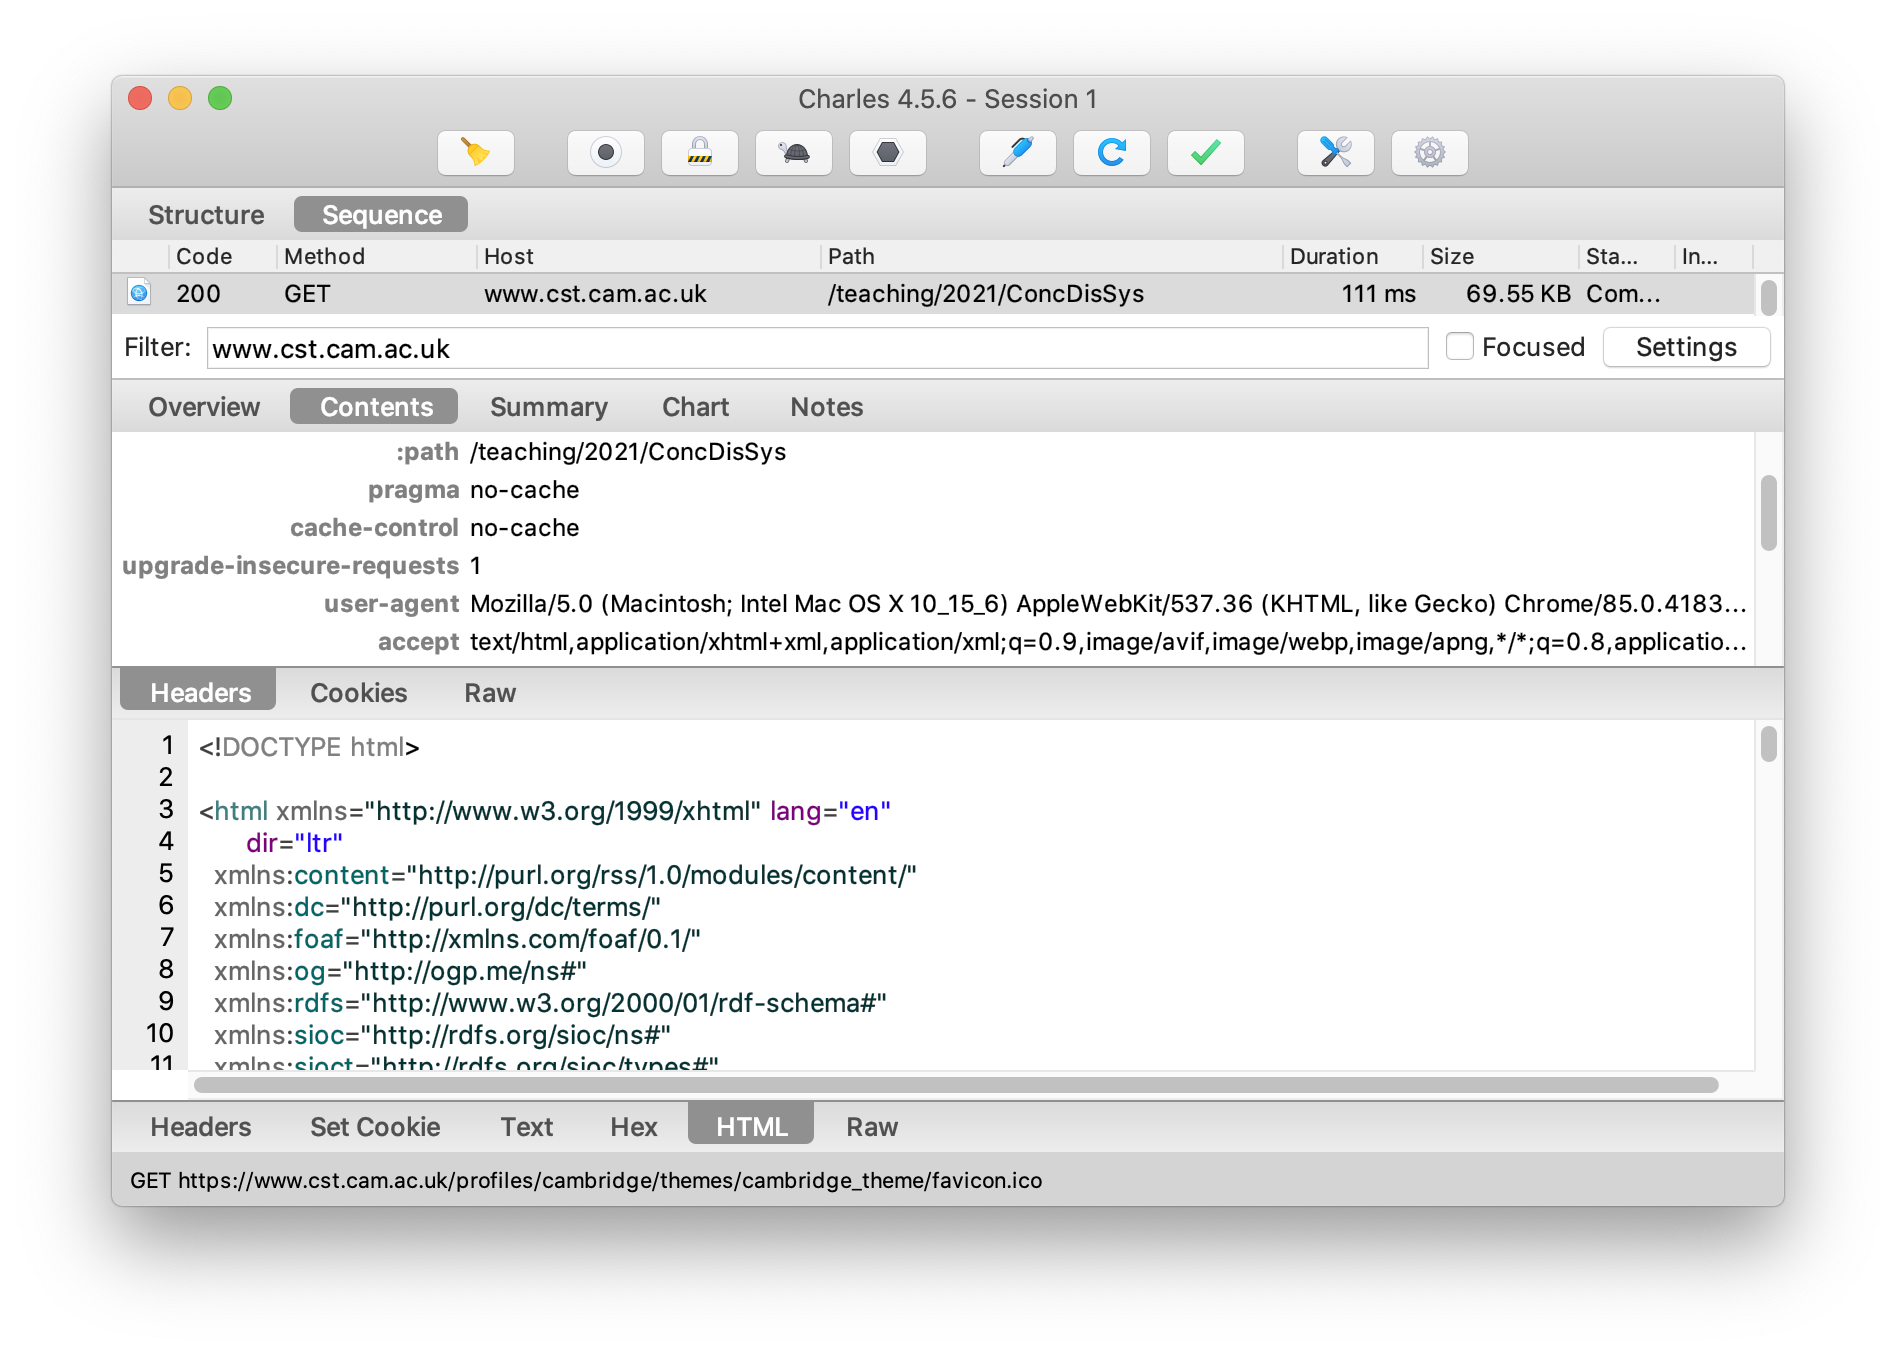
\includegraphics[height=8cm]{images/http-capture.png}};
        \node<2> (request) at (-4,-4.5) [red] {request message};
        \node<2> (response) at (2,-4.5) [red] {response message};
        \draw<2> [-Stealth,red,line width=4pt] (request) -- (-4,0.5);
        \draw<2> [-Stealth,red,line width=4pt] (response) -- (0,-1.2);
    \end{tikzpicture}
\end{frame}
\inlineslide{s:http-capture}\label{l:http-capture}

In a URL, the part between the \verb|//| and the following \verb|/| is the hostname of the server to which the client is going to send the request (e.g.\ \texttt{www.cst.cam.ac.uk}), and the rest (e.g.\ \texttt{\coursepath}) is the path that the client asks for in its request message.
Besides the path, the request also contains some extra information, such as the HTTP method (e.g.\ \texttt{GET} to load a page, or \texttt{POST} to submit a form), the version of the client software (the \emph{user-agent}), and a list of file formats that the client understands (the \emph{accept header}).
The response message contains the file that was requested, and an indicator of its file format (the \emph{content-type}); in the case of a web page, this might be a HTML document, an image, a video, a PDF document, or any other type of file.

Since the requests and responses can be larger than we can fit in a single network packet, the HTTP protocol runs on top of TCP, which breaks down a large chunk of data into a stream of small network packets (see \autoref{l:wireshark}), and puts them back together again at the recipient.
HTTP also allows multiple requests and multiple responses to be sent over a single TCP connection.
However, when looking at this protocol from a distributed systems point of view, this detail is not important: we treat the request as one message and the response as another message, regardless of the number of physical network packets involved in transmitting them.
This keeps things independent of the underlying networking technology.

\begin{frame}[plain]
    \label{s:wireshark}
    \begin{tikzpicture}[remember picture,overlay]
        \node at (current page.center) {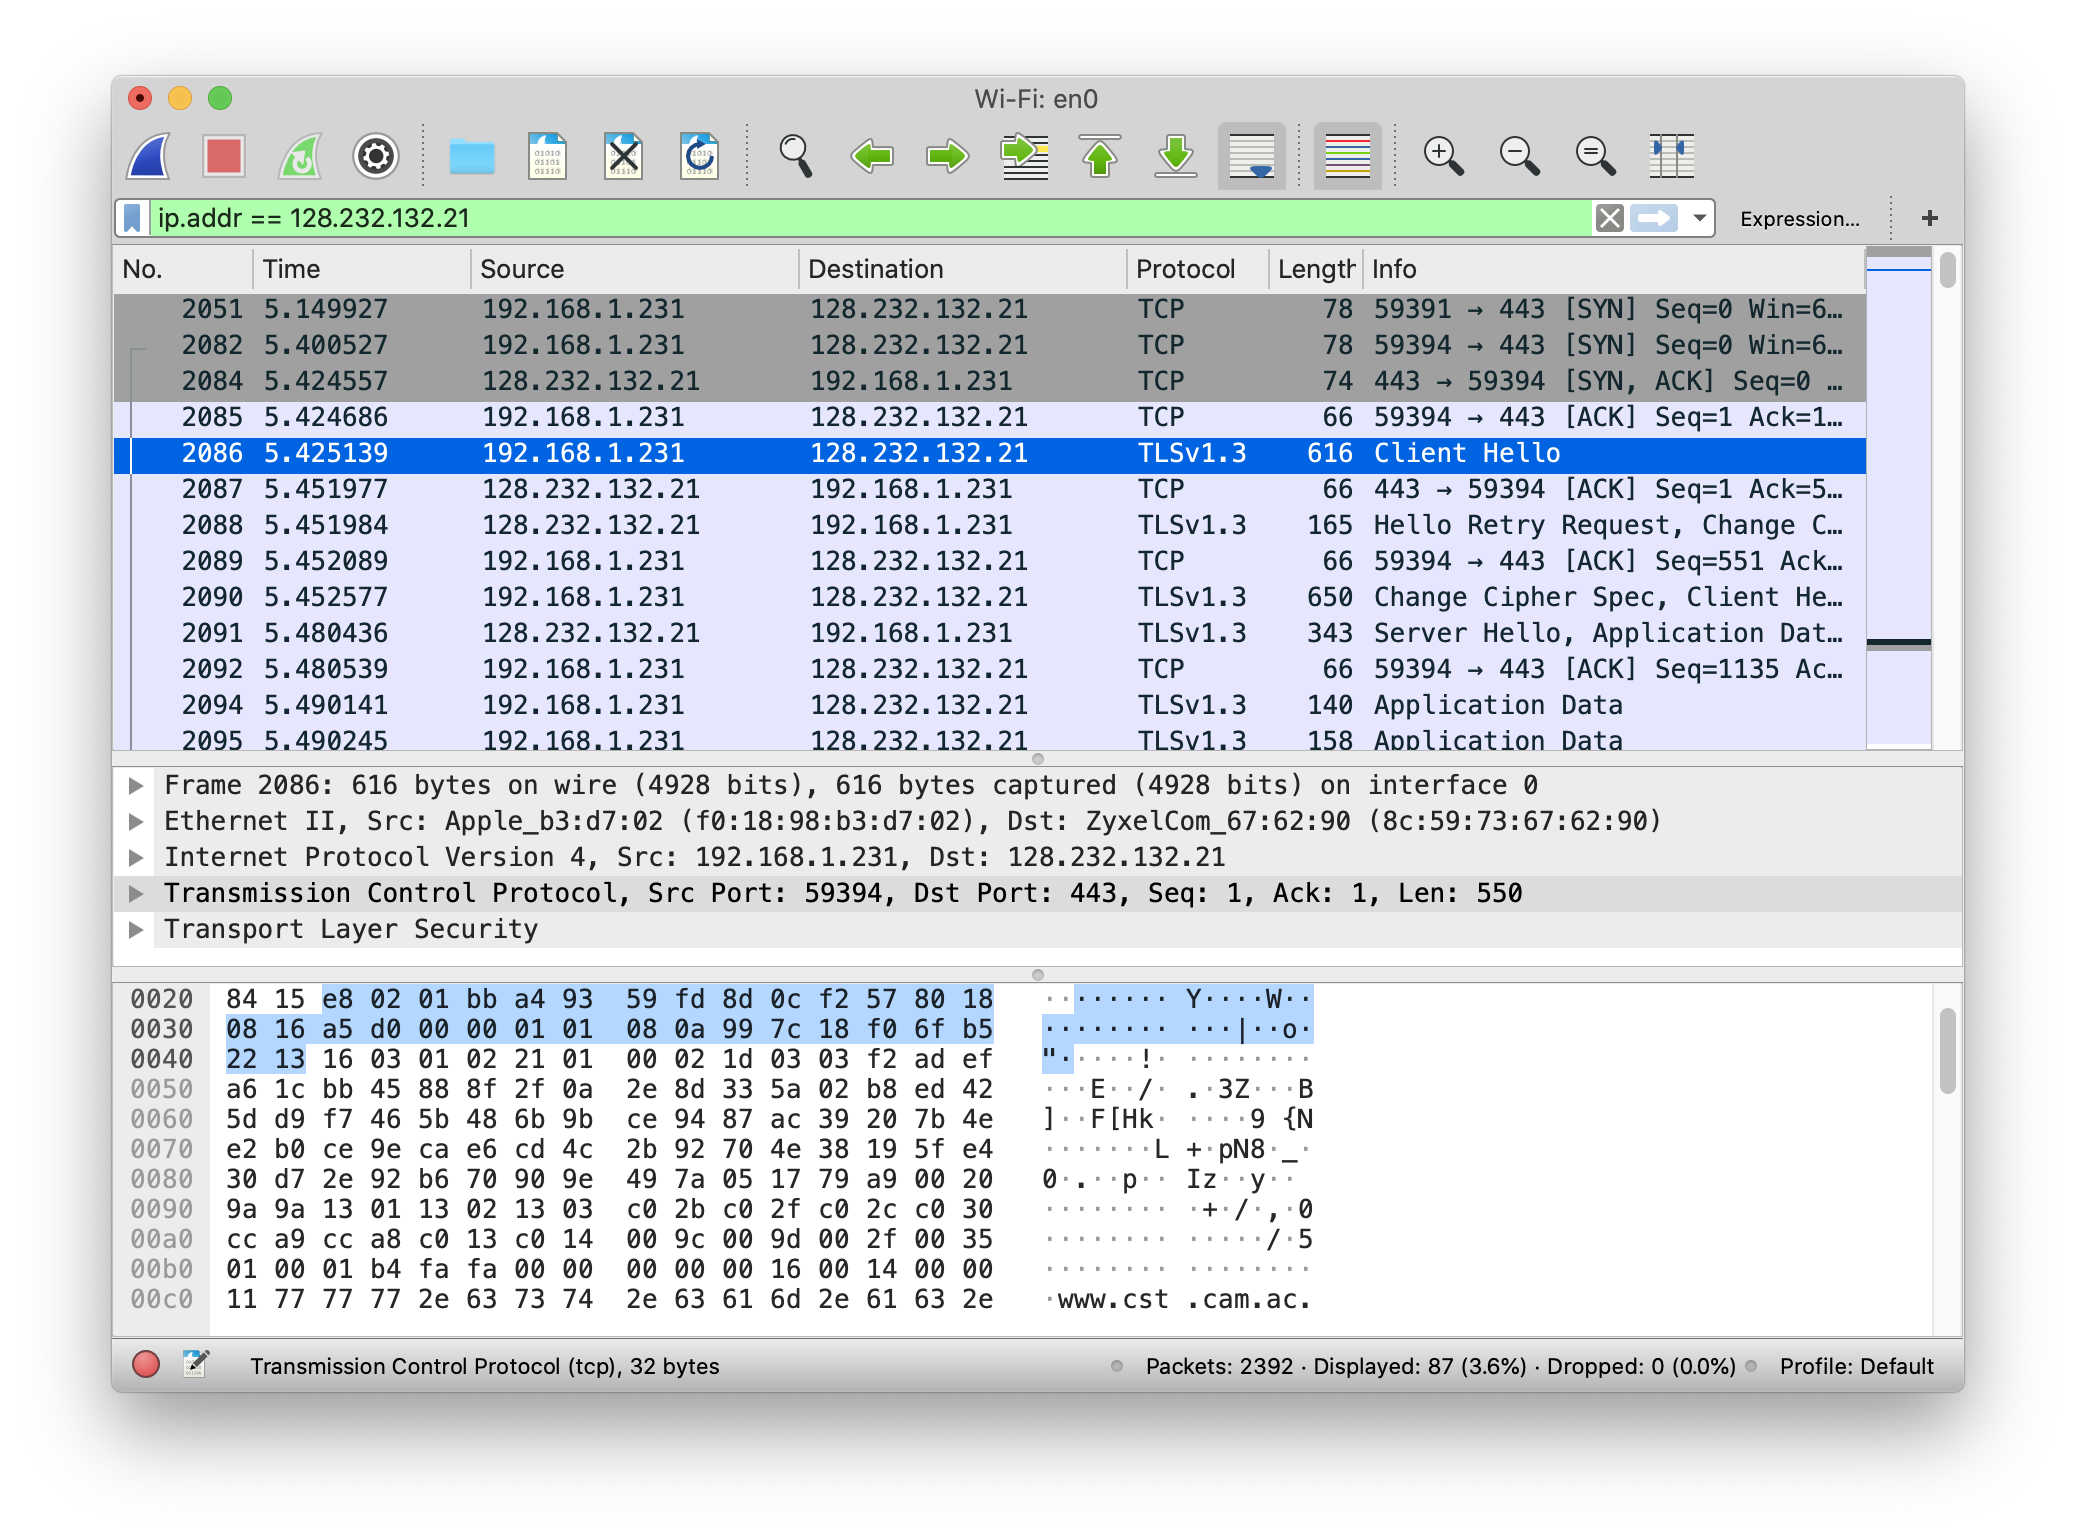
\includegraphics[height=\paperheight]{images/wireshark.png}};
    \end{tikzpicture}
\end{frame}
\inlineslide{s:wireshark}\label{l:wireshark}

\subsection{Example: remote procedure calls (RPC)}\label{sec:rpc}

Another example of an everyday distributed system is when you buy something online using a credit/debit card.
When you enter your card number in some online shop, that shop will send a payment request over the Internet to a service that specialises in processing card payments.

\begin{frame}
    \label{s:payment-example}
    \frametitle{Client-server example: online payments}
    \begin{center}
        \begin{tikzpicture}
            \node [rectangle,fill=red!10,draw] (client) at (0,4) {online shop};
            \node [rectangle,fill=red!10,draw] (server) at (8,4) {payments service};
            \draw (client) -- (0,0);
            \draw (server) -- (8,0);
            \draw<2-> [bigarrow] (0,3) -- node [above,sloped] {charge {\textsterling}3.99 to credit card 1234\dots} (8,2);
            \draw<3> [bigarrow] (8,1.5) -- node [above,sloped] {success} (0,0.5);
        \end{tikzpicture}
    \end{center}
\end{frame}
\inlineslide{s:payment-example}

The payments service in turn communicates with a card network such as Visa or MasterCard, which communicates with the bank that issued your card in order to take the payment.

For the programmers who are implementing the online shop, the code for processing the payment may look something like the code on \autoref{l:payment-rpc}.

\begin{frame}
    \label{s:payment-rpc}
    \frametitle{Remote Procedure Call (RPC) example}
    \inputminted{java}{code/payment-rpc.java}
    \begin{tikzpicture}[remember picture,overlay]
        \node (call) [xshift=2cm,yshift=-0.5cm] at (current page.center) {};
        \node<2> (label) [anchor=south east,red,yshift=0.5cm] at (current page.south east) {Implementation of this function is on another node!};
        \draw<2> [-Stealth,red,line width=4pt] (label) -- (call);
    \end{tikzpicture}
\end{frame}
\inlineslide{s:payment-rpc}\label{l:payment-rpc}

Calling the \verb|processPayment| function looks like calling any other function, but in fact, what is happening behind the scenes is that the shop is sending a request to the payments service, waiting for a response, and then returning the response it received.
The actual implementation of \verb|processPayment|~-- the logic that communicates with the card network and the banks~-- does not exist in the code of the shop: it is part of the payments service, which is another program running on another node belonging to a different company.

This type of interaction, where code on one node appears to call a function on another node, is called a \emph{Remote Procedure Call} (RPC).
In Java, it is called \emph{Remote Method Invocation} (RMI).
The software that implements RPC is called an \emph{RPC framework} or \emph{middleware}.
(Not all middleware is based on RPC; there is also middleware that uses different communication models.)

When an application wishes to call a function on another node, the RPC framework provides a \emph{stub} in its place.
The stub has the same type signature as the real function, but instead of executing the real function, it encodes the function arguments in a message and sends that message to the remote node, asking for that function to be called.
The process of encoding the function arguments is known as \emph{marshalling}.
In the example on \autoref{l:payment-json}, a JSON encoding is used for marshalling, but various other formats are also used in practice.

\begin{frame}[plain]
    \label{s:payment-json}
    \hspace*{-1cm}
    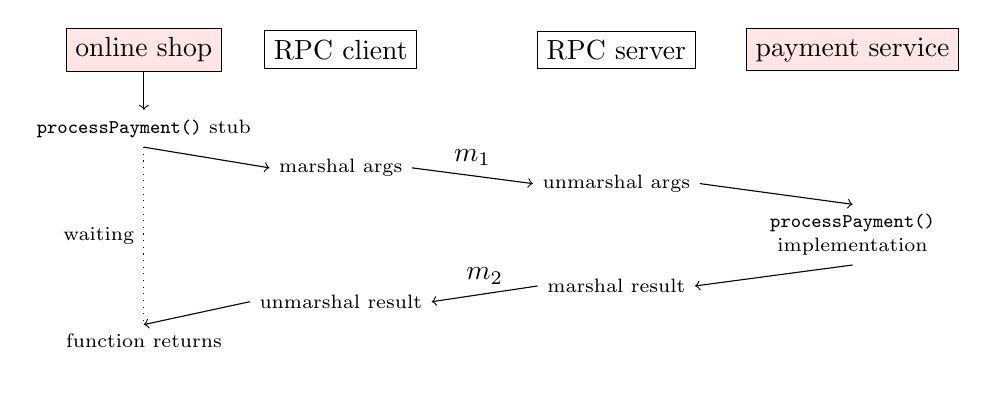
\begin{tikzpicture}
        \node [rectangle,fill=red!10,draw] (client) at (0,4) {online shop};
        \node [rectangle,draw] (rpc-client) at (2.5,4) {RPC client};
        \node [rectangle,draw] (rpc-server) at (6,4) {RPC server};
        \node [rectangle,fill=red!10,draw] (server) at (9,4) {payment service};
        \node [font=\scriptsize] (invoke) at (0,3) {\texttt{processPayment()} stub};
        \draw [->] (client) -- (invoke);
        \node<2-> [font=\scriptsize] (send-req) at (2.5,2.5) {marshal args};
        \draw<2-> [->] (invoke.south) -- (send-req.west);
        \node<2-> [font=\scriptsize] (recv-req) at (6,2.3) {unmarshal args};
        \draw<2-> [->] (send-req.east) -- node [above] {$m_1$} (recv-req.west);
        \node<3-> [font=\scriptsize] (exec) at (9,1.8) {\texttt{processPayment()}};
        \node<3-> [font=\scriptsize] (exec2) at (9,1.5) {implementation};
        \draw<3-> [->] (recv-req.east) -- (exec.north);
        \node<4-> [font=\scriptsize] (send-res) at (6,1) {marshal result};
        \draw<4-> [->] (exec2.south) -- (send-res.east);
        \node<4-> [font=\scriptsize] (recv-res) at (2.5,0.8) {unmarshal result};
        \draw<4-> [->] (send-res.west) -- node [above] {$m_2$} (recv-res.east);
        \node<5> [font=\scriptsize] (return) at (0,0.3) {function returns};
        \draw<5> [->] (recv-res.west) -- (return.north);
        \draw [dotted] (invoke.south) -- node [left,font=\scriptsize] {waiting} (0,0.5);
        \node at (0,0) {}; % so that messages below stay put as the slide builds
    \end{tikzpicture}
    \hspace*{-1cm}\mbox{
        \onslide<2->{
            $m_1$ = \begin{minipage}{5.5cm}
            \inputminted[fontsize=\scriptsize,frame=single,bgcolor=lightgrey]{json}{code/payment-rpc.json}
            \end{minipage}
        }
        \onslide<4->{
            $m_2$ = \begin{minipage}{3.8cm}
            \inputminted[fontsize=\scriptsize,frame=single,bgcolor=lightgrey]{json}{code/payment-response.json}
            \end{minipage}
        }
    }
\end{frame}
\inlineslide{s:payment-json}\label{l:payment-json}

The sending of the message from the RPC client to the RPC server may happen over HTTP (in which case this is also called a \emph{web service}), or one of a range of different network protocols may be used.
On the server side, the RPC framework unmarshals (decodes) the message and calls the desired function with the provided arguments.
When the function returns, the same happens in reverse: the function's return value is marshalled, sent as a message back to the client, unmarshalled by the client, and returned by the stub.
Thus, to the caller of the stub, it looks as if the function had executed locally.

\begin{frame}
    \label{s:rpc-problems}
    \frametitle{Remote Procedure Call (RPC)}
    Ideally, RPC makes a call to a remote function look the same as a local function call.\\[1em]
    \textbf{``Location transparency''}:\\ system hides where a resource is located.\\[1em]\pause
    In practice\dots
    \begin{itemize}
        \item what if the service crashes during the function call?
        \item what if a message is lost?
        \item what if a message is delayed?
        \item if something goes wrong, is it safe to retry?
    \end{itemize}
\end{frame}
\inlineslide{s:rpc-problems}

\supervision{
    Networks and nodes might fail.
    What are the implications for code that calls another node through RPC?
    How is RPC different from a local function call?
    Is location transparency achievable?
}{
    \begin{itemize}
        \item RPCs may time out if the request or response message is lost.
            Even if we retry, there is no guarantee that the messages will get through.
            The application must handle this error condition, and the possibility of failure may need to be reflected in the type signature.
            For example, Java RPC libraries often throw a checked exception, and JavaScript RPC clients often return a \emph{promise}, which can either succeed or fail.
        \item If a timeout occurs, the RPC client doesn't know whether the server executed the function; local function calls don't have this uncertainty.
        \item RPC is often much slower than a local function call, due to network latency.
            Moreover, network latency is often variable and unpredictable, while the execution speed of a local function is usually predictable.
        \item RPC clients and servers may need to take measures to make function invocation idempotent, to allow safe retries in case of message loss.
        \item Perfect location transparency can only be achieved by making local function calls more like RPCs (e.g.\ allowing them to unpredictably fail).
            This is undesirable in most cases, and therefore most systems do not attempt to completely hide the distinction between local and remote calls.
    \end{itemize}
}

Over the decades many variants of RPC have been developed, with the goal of making it easier to program distributed systems.
This includes object-oriented middleware such as CORBA in the 1990s.
However, the underlying distributed systems challenges have remained the same \citep{Waldo:1994wx}.

\begin{frame}
    \label{s:rpc-history}
    \frametitle{RPC history}
    \begin{itemize}
        \item SunRPC/ONC RPC (1980s, basis for NFS)
        \item CORBA: object-oriented middleware, hot in the 1990s
        \item Microsoft's DCOM and Java RMI (similar to CORBA)
        \item SOAP/XML-RPC: RPC using XML and HTTP (1998)
        \item Thrift (Facebook, 2007)
        \item gRPC (Google, 2015)
        \item REST (often with JSON)
        \item Ajax in web browsers
    \end{itemize}
\end{frame}
\inlineslide{s:rpc-history}

Today, the most common form of RPC is implemented using JSON data sent over HTTP.
A popular set of design principles for such HTTP-based APIs is known as \emph{representational state transfer} or \emph{REST} \citep{Fielding:2000}, and APIs that adhere to these principles are called \emph{RESTful}.
These principles include:
\begin{itemize}
    \item communication is stateless (each request is self-contained and independent from other requests),
    \item resources (objects that can be inspected and manipulated) are represented by URLs, and
    \item the state of a resource is updated by making a HTTP request with a standard method type, such as \texttt{POST} or \texttt{PUT}, to the appropriate URL.
\end{itemize}
The popularity of REST is due to the fact that JavaScript code running in a web browser can easily make this type of HTTP request, as shown in \autoref{l:javascript-rpc}.
In modern websites it is very common to use JavaScript to make HTTP requests to a server without reloading the whole page.
This technique is sometimes known as \emph{Ajax}.

\begin{frame}
    \label{s:javascript-rpc}
    \frametitle{RPC/REST in JavaScript}
    \inputminted{js}{code/payment-rpc.js}
\end{frame}
\inlineslide{s:javascript-rpc}\label{l:javascript-rpc}

The code on \autoref{l:javascript-rpc} takes the arguments \verb|args|, marshals them to JSON using \verb|JSON.stringify()|, and then sends them to the URL \verb|https://example.com/payments| using a HTTP POST request.
There are three possible outcomes: either the server returns a status code indicating success (in which case we unmarshal the response using \verb|response.json()|), or the server returns a status code indicating an error, or the request fails because no response was received from the server (most likely due to a network interruption).
The code calls either the \verb|success()| or the \verb|failure()| function in each of these cases.

Even though RESTful APIs and HTTP-based RPC originated on the web (where the client is JavaScript running in a web browser), they are now also commonly used with other types of client (e.g.\ mobile apps), or for server-to-server communication.

\begin{frame}
    \label{s:rpc-discussion}
    \frametitle{RPC in enterprise systems}
    \textbf{``Service-oriented architecture''} (SOA) / ``microservices'':\\[1em]
    splitting a large software application into multiple services\\ (on multiple nodes) that communicate via RPC.\\[1.5em]\pause

    Different services implemented in different languages:
    \begin{itemize}
        \item interoperability: datatype conversions
        \item \textbf{Interface Definition Language} (IDL): language-independent API specification
    \end{itemize}
\end{frame}
\inlineslide{s:rpc-discussion}

Such server-to-server RPC is especially common in large enterprises, whose software systems are too large and complex to run in a single process on a single machine.
To manage this complexity, the system is broken down into multiple services, which are developed and administered by different teams and which may even be implemented in different programming languages.
RPC frameworks facilitate the communication between these services.

When different programming languages are used, the RPC framework needs to convert datatypes such that the caller's arguments are understood by the code being called, and likewise for the function's return value.
A typical solution is to use an \emph{Interface Definition Language} (IDL) to provide language-independent type signatures of the functions that are being made available over RPC.
From the IDL, software developers can then automatically generate marshalling/unmarshalling code and RPC stubs for the respective programming languages of each service and its clients.
\autoref{l:rpc-idl} shows an example of the IDL used by gRPC, called \emph{Protocol Buffers}.
The details of the language are not important for this course.

\begin{frame}
    \label{s:rpc-idl}
    \frametitle{gRPC IDL example}
    \inputminted[fontsize=\scriptsize]{protobuf}{code/payment-rpc.proto}
\end{frame}
\inlineslide{s:rpc-idl}\label{l:rpc-idl}

% If the client sends the RPC request but receives no response, it doesn't know whether or not the server received and processed the request.
% It could resend the request if it doesn't hear back for a while, but that might cause the request to be performed more than once (e.g.\ charging a credit card twice), unless we take care to make the request idempotent.
% But even if we retry, there is no guarantee that the retried messages will get through either.
%
% Waiting forever is not a good approach, so in practice we have to give up after some timeout.
% As the client has not received a response, the RPC stub will not be able to return a value of the function's return type, but rather it will need to somehow indicate to the calling code that a timeout occurred, e.g.\ by throwing an exception.

\section{Models of distributed systems}

A \emph{system model} captures our assumptions about how nodes and the network behave.
It is an abstract description of their properties, which can be implemented by various technologies in practice.
To illustrate common system models, we will start this section by looking at two classic thought experiments in distributed systems: the \emph{two generals problem} and the \emph{Byzantine generals problem}.

\subsection{The two generals problem}

In the two generals problem \citep{Gray:1978}, we imagine two generals, each leading an army, who want to capture a city.
(Apologies for the militaristic analogy~-- I didn't come up with it!)
The city's defences are strong, and if only one of the two armies attacks, the army will be defeated.
However, if both armies attack at the same time, they will successfully capture the city.

\begin{frame}
    \label{s:two-generals}
    \frametitle{The two generals problem}
    \begin{center}
        \begin{tikzpicture}
            \node [rectangle,fill=red!10,draw] (army1) at (0,0) {army 1};
            \node [rectangle,fill=red!10,draw] (army2) at (8,0) {army 2};
            \node [circle,fill=blue!10,draw] (city) at (4,2) {city};
            \draw [thick,dashed,-{Stealth[length=3mm]}] (army1) -- node [left,yshift=0.2cm] {attack?} (city);
            \draw [thick,dashed,-{Stealth[length=3mm]}] (army2) -- node [right,yshift=0.2cm] {attack?} (city);
            \draw [doublebigarrow] (army1) -- node [below] {messengers} (army2);
        \end{tikzpicture}\\[1.5em]\pause
        \begin{tabular}{|c|c|c|}
            \hline
            army 1 & army 2 & outcome \\\hline
            does not attack & does not attack & nothing happens \\
            attacks & does not attack & army 1 defeated \\
            does not attack & attacks & army 2 defeated \\
            attacks & attacks & city captured \\\hline
        \end{tabular}\\[1.5em]
        \textbf{Desired:} army 1 attacks \emph{if and only if} army 2 attacks
    \end{center}
\end{frame}
\inlineslide{s:two-generals}\label{l:two-generals}

Thus, the two generals need to coordinate their attack plan.
This is made difficult by the fact that the two armies are camped some distance apart, and they can only communicate by messenger.
The messengers must pass through territory controlled by the city, and so they are sometimes captured.
Thus, a message sent by one general may or may not be received by the other general, and the sender does not know whether their message got through, except by receiving an explicit reply from the other party.
If a general does not receive any messages, it is impossible to tell whether this is because the other general didn't send any messages, or because all messengers were captured.

\begin{frame}
    \label{s:two-generals-comms}
    \frametitle{The two generals problem}
    \begin{center}
        \begin{tikzpicture}
            \node [rectangle,fill=red!10,draw] (gen1) at (0,3) {general 1};
            \node [rectangle,fill=red!10,draw] (gen2) at (8,3) {general 2};
            \draw (gen1) -- (0,0);
            \draw (gen2) -- (8,0);
            \draw [bigarrow] (0,2.2) -- node [above,sloped] {attack 10 Nov, okay?} (8,1.2);
            \draw [messageloss] (8,0.7) -- node [above,sloped] {10 Nov agreed!} (2,0);
        \end{tikzpicture}\pause\\[1em]
        From general 1's point of view, this is indistinguishable from:\\[1em]
        \begin{tikzpicture}
            \node [rectangle,fill=red!10,draw] (gen1) at (0,3) {general 1};
            \node [rectangle,fill=red!10,draw] (gen2) at (8,3) {general 2};
            \draw (gen1) -- (0,1);
            \draw (gen2) -- (8,1);
            \draw [messageloss] (0,2.2) -- node [above,sloped] {attack 10 Nov, okay?} (6,1.4);
        \end{tikzpicture}
    \end{center}
\end{frame}
\inlineslide{s:two-generals-comms}

What protocol should the two generals use to agree on a plan?
For each general there are two options: either the general promises to go ahead with the attack in any case (even if no response is received), or the general waits for an acknowledgement before committing to attack.
In the first case, the general who promises to go ahead risks being alone in the attack.
In the second case, the general who awaits acknowledgement shifts the problem to the other general, who must now decide whether to commit to attack (and risk being alone) or wait for an acknowledgement of the acknowledgement.

\begin{frame}
    \label{s:two-generals-proto}
    \frametitle{How should the generals decide?}
    \begin{enumerate}
        \item General 1 always attacks, even if no response is received?
            \begin{itemize}
                \item Send lots of messengers to increase probability that one will get through
                \item If all are captured, general 2 does not know about the attack, so general 1 loses\\[1em]\pause
            \end{itemize}
        \item General 1 only attacks if positive response from general 2 is received?
            \begin{itemize}
                \item Now general 1 is safe
                \item But general 2 knows that general 1 will only attack if general 2's response gets through
                \item Now general 2 is in the same situation as general 1 in option 1\\[0.5em]\pause
            \end{itemize}
    \end{enumerate}
    \textbf{No common knowledge}: the only way of knowing something is to communicate it
\end{frame}
\inlineslide{s:two-generals-proto}

The problem is that no matter how many messages are exchanged, neither general can ever be certain that the other army will also turn up at the same time.
A repeated sequence of back-and-forth acknowledgements can build up gradually increasing confidence that the generals are in agreement, but it can be proved that they cannot reach certainty by exchanging any finite number of messages.

This thought experiment demonstrates that in a distributed system, there is no way for one node to have certainty about the state of another node.
The only way how a node can know something is by having that knowledge communicated in a message.
On a philosophical note, this is perhaps similar to communication between humans: we have no telepathy, so the only way for someone else to know what you are thinking is by communicating it (through speech, writing, body language, etc).

As a practical example of the two generals problem, \autoref{l:two-generals-applied} adapts the model from \autoref{l:two-generals} to the application of paying for goods in an online shop.
The shop and the credit card payment processing service communicate per RPC, and some of these messages may be lost.
Nevertheless, the shop wants to ensure that it dispatches the goods only if they are paid for, and it only charges the customer card if the goods are dispatched.

\begin{frame}
    \label{s:two-generals-applied}
    \frametitle{The two generals problem applied}
    \begin{center}
        \begin{tikzpicture}
            \node [rectangle,fill=red!10,draw] (army1) at (0,0) {online shop};
            \node [rectangle,fill=red!10,draw] (army2) at (8,0) {payments service};
            \node [circle,fill=blue!10,draw] (city) at (4,2) {customer};
            \draw [thick,dashed,-{Stealth[length=3mm]}] (army1) -- node [left,yshift=0.2cm] {dispatch goods} (city);
            \draw [thick,dashed,-{Stealth[length=3mm]}] (army2) -- node [right,yshift=0.2cm] {charge credit card} (city);
            \draw [doublebigarrow] (army1) -- node [below] {RPC} (army2);
        \end{tikzpicture}\\[1.5em]\pause
        \begin{tabular}{|c|c|c|}
            \hline
            online shop & payments service & outcome \\\hline
            does not dispatch & does not charge & nothing happens \\
            dispatches & does not charge & shop loses money \\
            does not dispatch & charges & customer complaint \\
            dispatches & charges & everyone happy \\\hline
        \end{tabular}\\[1.5em]
        \textbf{Desired:} online shop dispatches \emph{if and only if} payment made
    \end{center}
\end{frame}
\inlineslide{s:two-generals-applied}\label{l:two-generals-applied}

In practice, systems such as online shops work around the two generals problem in various pragmatic ways: for example, by periodically reconciling transaction records with the payments service, checking the status of transactions that timed out due to a network problem, and by reimbursing any orders that could not be fulfilled.
Just because the two generals problem cannot be solved, that does not mean the challenges it raises are insurmountable: it just means that we have to think carefully and creatively about the problem.

\subsection{The Byzantine generals problem}

The Byzantine generals problem \citep{Lamport:1982} has a similar setting to the two generals problem.
Again we have armies wanting to capture a city, though in this case there can be three or more.
Again generals communicate by messengers, although this time we assume that if a message is sent, it is always delivered correctly.

\begin{frame}
    \label{s:byzantine-generals}
    \frametitle{The Byzantine generals problem}
    \begin{center}
        \begin{tikzpicture}
            \node [rectangle,fill=red!10,draw] (army1) at (0,0) {army 1};
            \node [rectangle,fill=red!10,draw] (army2) at (8,0) {army 2};
            \node [rectangle,fill=red!10,draw] (army3) at (4,5.5) {army 3};
            \node [circle,fill=blue!10,draw] (city) at (4,2.5) {city};
            \draw [thick,dashed,-{Stealth[length=3mm]}] (army1) -- node [right,yshift=-0.2cm] {attack?} (city);
            \draw [thick,dashed,-{Stealth[length=3mm]}] (army2) -- node [left,yshift=-0.2cm] {attack?} (city);
            \draw [thick,dashed,-{Stealth[length=3mm]}] (army3) -- node [left,yshift=-0.4cm] {attack?} (city);
            \draw [doublebigarrow] (army1.east)  -- node [below] {messengers} (army2.west);
            \draw [doublebigarrow] (army1.north) -- node [left]  {messengers} (army3.south west);
            \draw [doublebigarrow] (army2.north) -- node [right] {messengers} (army3.south east);
        \end{tikzpicture}\\[1.5em]
        \textbf{Problem:} some of the generals might be traitors
    \end{center}
\end{frame}
\inlineslide{s:byzantine-generals}\label{l:byzantine-generals}

The challenge in the Byzantine setting is that some generals might be ``traitors'': that is, they might try to deliberately and maliciously mislead and confuse the other generals.
One example of such malicious behaviour is shown on \autoref{l:byzantine-generals-comms}: here, general 3 receives two contradictory messages from generals 1 and 2.
General 1 tells general 3 to attack, whereas general 2 claims that general 1 ordered a retreat.
It is impossible for general 3 to determine whether general 2 is lying (the first case), or whether general 2 is honest while general 1 is issuing contradictory orders (the second case).

\begin{frame}
    \label{s:byzantine-generals-comms}
    \frametitle{Generals that might lie}
    \begin{center}
        \begin{tikzpicture}
            \node [rectangle,fill=red!10,draw] (gen1) at (0,2.6) {general 1};
            \node [rectangle,fill=red!10,draw] (gen2) at (4.5,2.6) {general 2};
            \node [rectangle,fill=red!10,draw] (gen3) at (9,2.6) {general 3};
            \draw (gen1) -- (0,0);
            \draw (gen2) -- (4.5,0);
            \draw (gen3) -- (9,0);
            \draw [bigarrow] (0,2.0) -- node [above,sloped,pos=0.25] {attack!} (9,1.2);
            \draw [bigarrow] (0,1.3) -- node [above,sloped] {attack!} (4.5,0.9);
            \draw [bigarrow] (4.5,0.6) -- node [above,sloped] {general 1 said retreat!} (9,0.2);
        \end{tikzpicture}\pause\\[1em]
        From general 3's point of view, this is indistinguishable from:\\[1em]
        \begin{tikzpicture}
            \node [rectangle,fill=red!10,draw] (gen1) at (0,2.6) {general 1};
            \node [rectangle,fill=red!10,draw] (gen2) at (4.5,2.6) {general 2};
            \node [rectangle,fill=red!10,draw] (gen3) at (9,2.6) {general 3};
            \draw (gen1) -- (0,0);
            \draw (gen2) -- (4.5,0);
            \draw (gen3) -- (9,0);
            \draw [bigarrow] (0,2.0) -- node [above,sloped,pos=0.25] {attack!} (9,1.2);
            \draw [bigarrow] (0,1.3) -- node [above,sloped] {retreat!} (4.5,0.9);
            \draw [bigarrow] (4.5,0.6) -- node [above,sloped] {general 1 said retreat!} (9,0.2);
        \end{tikzpicture}
    \end{center}
\end{frame}
\inlineslide{s:byzantine-generals-comms}\label{l:byzantine-generals-comms}

The honest generals don't know who the malicious generals are, but the malicious generals may collude and secretly coordinate their actions.
We might even assume that all of the malicious generals are controlled by an evil adversary.
The Byzantine generals problem is then to ensure that all honest generals agree on the same plan (e.g.\ whether to attack or to retreat).
It is impossible to specify what the malicious generals are going to do, so the best we can manage is to get the honest generals to agree.

This is difficult: in fact, it can be proved that some variants of the problem can be solved only if strictly fewer than one third of the generals are malicious.
That is, in a system with $3f+1$ generals, no more than $f$ may be malicious.
For example, a system with 4 generals can tolerate $f=1$ malicious general, and a system with 7 generals can tolerate $f=2$.

\begin{frame}
    \label{s:byzantine-discussion}
    \frametitle{The Byzantine generals problem}
    \begin{itemize}
        \item Up to $f$ generals might behave malicously\\[0.5em]
        \item Honest generals don't know who the malicious ones are\\[0.5em]
        \item The malicious generals may collude\\[0.5em]
        \item Nevertheless, honest generals must agree on plan\\[2em]\pause
        \item Theorem: need $3f+1$ generals in total to tolerate $f$ malicious generals (i.e.\ $< \frac{1}{3}$ may be malicious)\\[0.5em]
        \item Cryptography (digital signatures) helps~-- but problem remains hard\\[0.5em]
    \end{itemize}
\end{frame}
\inlineslide{s:byzantine-discussion}

The problem is made somewhat easier if generals use cryptography (\emph{digital signatures}) to prove who said what: for example, this would allow general 2 to prove to general 3 what general 1's order was, and thus demonstrate general 2's honesty.
We will not go into details of digital signatures in this course, as they are covered in the Security course (Part IB Easter term).
However, even with signatures, the Byzantine generals problem remains challenging.

Is the Byzantine generals problem of practical relevance?
Real distributed systems do often involve complex trust relationships.
For example, a customer needs to trust an online shop to actually deliver the goods they ordered, although they can dispute the payment via their bank if the goods never arrive or if they get charged too much.
But if an online shop somehow allowed customers to order goods without paying for them, this weakness would no doubt be exploited by fraudsters, so the shop must assume that customers are potentially malicious.
On the other hand, for RPC between services belonging to the shop, running in the same datacentre, one service can probably trust the other services run by the same company.
The payments service doesn't fully trust the shop, since someone might set up a fraudulent shop or use stolen credit card numbers, but the shop probably does trust the payments service.
And so on.
And in the end, we want the customer, the online shop, and the payments service to agree on any order that is placed.
The Byzantine generals problem is a simplification of such complex trust relationships, but it is a good starting point for studying systems in which some participants might behave maliciously.

\begin{frame}
    \label{s:byzantine-payment}
    \frametitle{Trust relationships and malicious behaviour}
    \begin{center}
        \begin{tikzpicture}
            \node [rectangle,fill=red!10,draw] (army1) at (0,0) {online shop};
            \node [rectangle,fill=red!10,draw] (army2) at (8,0) {payments service};
            \node [rectangle,fill=red!10,draw] (army3) at (4,5.5) {customer};
            \node [circle,fill=blue!10,draw] (city) at (4,2.5) {order};
            \draw [thick,dashed,-{Stealth[length=3mm]}] (army1) -- node [right,yshift=-0.2cm] {agree?} (city);
            \draw [thick,dashed,-{Stealth[length=3mm]}] (army2) -- node [left,yshift=-0.2cm] {agree?} (city);
            \draw [thick,dashed,-{Stealth[length=3mm]}] (army3) -- node [left,yshift=-0.4cm] {agree?} (city);
            \draw [doublebigarrow] (army1.east)  -- node [below] {RPC} (army2.west);
            \draw [doublebigarrow] (army1.north) -- node [left]  {RPC} (army3.south west);
            \draw [doublebigarrow] (army2.north) -- node [right] {RPC} (army3.south east);
        \end{tikzpicture}\\[1.5em]
        Who can trust whom?
    \end{center}
\end{frame}
\inlineslide{s:byzantine-payment}\label{l:byzantine-payment}

Before we move on, a brief digression about the origin of the word ``Byzantine''.
The term comes from the Byzantine empire, named after its capital city Byzantium or Constantinople, which is now Istanbul in Turkey.
There is no historical evidence that the generals of the Byzantine empire were any more prone to intrigue and conspiracy than those elsewhere.
Rather, the word \emph{Byzantine} had been used in the sense of ``excessively complicated, bureaucratic, devious'' long before Leslie Lamport adopted the word to describe the Byzantine generals problem; the exact etymology is unclear.

\pagebreak[3]
\begin{frame}
    \label{s:byzantine-empire}
    \frametitle{The Byzantine empire (650 CE)}
    \begin{tikzpicture}
        \node at (0,0) {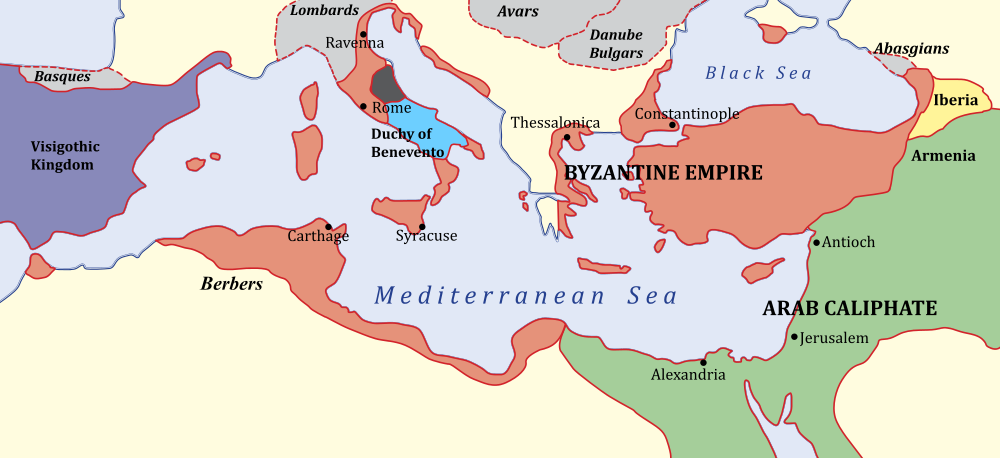
\includegraphics[height=5cm]{images/byzantium650.png}};
        \node (byzantium) at (2.4,3) {Byzantium/Constantinople/Istanbul};
        \draw<2> [-Stealth,line width=4pt] (byzantium) -- (1.9,1.2);
    \end{tikzpicture}
    {\scriptsize Source: \url{https://commons.wikimedia.org/wiki/File:Byzantiumby650AD.svg}}\\[1em]
    \textbf{``Byzantine''} has long been used for ``excessively complicated, bureaucratic, devious'' (e.g.\ \emph{``the Byzantine tax law''})
\end{frame}
\inlineslide{s:byzantine-empire}\label{l:byzantine-empire}

\subsection{Describing nodes and network behaviour}

When designing a distributed algorithm, a \emph{system model} is how we specify our assumptions about what faults may occur.

\begin{frame}
    \label{s:system-model}
    \frametitle{System models}
    We have seen two thought experiments:
    \begin{itemize}
        \item Two generals problem: a model of networks
        \item Byzantine generals problem: a model of node behaviour
    \end{itemize}
    In real systems, both nodes and networks may be faulty!\\[2em]\pause
    Capture assumptions in a \textbf{system model} consisting of:
    \begin{itemize}
        \item Network behaviour (e.g.\ message loss)
        \item Node behaviour (e.g.\ crashes)
        \item Timing behaviour (e.g.\ latency)
    \end{itemize}
    Choice of models for each of these parts.
\end{frame}
\inlineslide{s:system-model}\label{l:system-model}

\begin{frame}
    \label{s:shark-bite}
    \frametitle{Networks are unreliable}
    % Source for network-cable.jpg: https://pixabay.com/photos/modem-antenna-wire-cable-router-5436144/
    % (Royalty-free, no attribution required)
    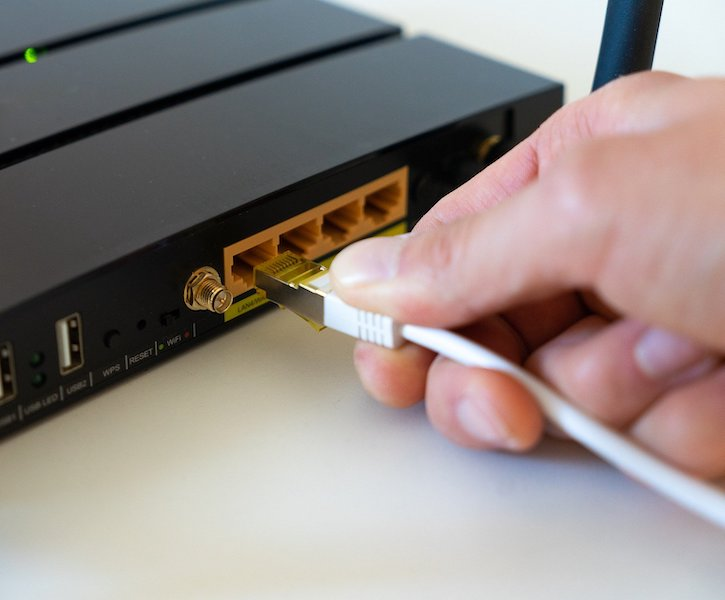
\includegraphics[height=4cm]{images/network-cable.jpg}
    
\includegraphics[height=4cm]{images/shark-bite.jpg}\\[1em]
    In the sea, sharks bite fibre optic cables \\
    {\scriptsize\url{https://slate.com/technology/2014/08/shark-attacks-threaten-google-s-undersea-internet-cables-video.html}}\\[1em]
    On land, cows step on the cables \\
    {\scriptsize\url{https://twitter.com/uhoelzle/status/1263333283107991558}}
\end{frame}
\inlineslide{s:shark-bite}\label{l:shark-bite}

Let's start with the network.
No network is perfectly reliable: even in carefully engineered systems with redundant network links, things can go wrong \citep{Bailis:2014jx}.
Someone might accidentally unplug the wrong network cable.
Sharks and cows have both been shown to cause damage and interruption to long-distance networks (see links on \autoref{l:shark-bite}).
Or a network may be temporarily overloaded, perhaps by accident or perhaps due to a denial-of-service attack.
Any of these can cause messages to be lost.

In a system model, we take a more abstract view, which saves us from the details of worrying about sharks and cows.
Most distributed algorithms assume that the network provides bidirectional message-passing between a pair of nodes, also known as \emph{point-to-point} or \emph{unicast} communication.
Real networks do sometimes allow \emph{broadcast} or \emph{multicast} communication (sending a packet to many recipients at the same time, which is used e.g.\ for discovering a printer on a local network), but broadly speaking, assuming unicast-only is a good model of the Internet today.
Later, in section TODO, we will show how to implement broadcast on top of unicast communication.

We can then choose how reliable we want to assume these links to be.
Most algorithms assume one of the three choices listed on \autoref{l:model-network}.

\begin{frame}
    \label{s:model-network}
    \frametitle{System model: network behaviour}
    Assume bidirectional \textbf{point-to-point} communication between two nodes, with one of:\pause
    \begin{itemize}
        \item \textbf{Reliable} (perfect) links:\\
            A message is received if and only if it is sent.\tikz[remember picture]\node (reliable) {};\\
            Messages may be reordered.\pause
        \item \textbf{Fair-loss} links:\\
            Messages may be lost, duplicated, or reordered.\tikz[remember picture]\node (fairloss) {};\\
            If you keep retrying, a message eventually gets through.\pause
        \item \textbf{Arbitrary} links (active adversary):\\
            A malicious adversary may interfere with messages\tikz[remember picture]\node (arbitrary) {};\\
            (eavesdrop, modify, drop, spoof, replay).\\[1em]
    \end{itemize}\pause
    \textbf{Network partition}: some links dropping/delaying all messages for extended period of time
    \begin{tikzpicture}[remember picture,overlay]
        \draw<6-> [-Stealth,red,line width=4pt] (fairloss.north) .. controls +(1.6,0) and +(1.6,0) ..
            node [right,red,align=left] {retry +\\dedup} (reliable);
        \draw<7> [-Stealth,red,line width=4pt] (arbitrary) .. controls +(1.6,0) and +(1.6,0) ..
            node [right,red,align=left] {TLS} (fairloss.south);
    \end{tikzpicture}
\end{frame}
\inlineslide{s:model-network}\label{l:model-network}

Interestingly, it is possible to convert some types of link into others.
For example, if we have a fair-loss link, we can turn it into a reliable link by continually retransmitting lost messages until they are finally received, and by filtering out duplicated messages on the recipient side.
The fair-loss assumption means that any \emph{network partition} (network interruption) will last only for a finite period of time, but not forever, so we can guarantee that every message will eventually be received.

Of course, any messages sent during a network partition will only be received after the interruption is repaired, which may take a long time, but the definitions on \autoref{l:model-network} do not say anything about network delay or latency.
We will get to that topic on \autoref{l:model-synchrony}.

The TCP protocol, which we discussed briefly in \autoref{sec:web}, performs this kind of retry and deduplication at the network packet level.
However, TCP is usually configured with a timeout, so it will give up and stop retrying after a certain time, typically on the order of one minute.
To overcome network partitions that last for longer than this duration, a separate retry and deduplication mechanism needs to be implemented in addition to that provided by TCP.

An arbitrary link is an accurate model for communication over the Internet: whenever your communication is routed through a network (be it a coffee shop wifi or an Internet backbone network), the operator of that network can potentially interfere with and manipulate your network packets in arbitrary ways.
Someone who manipulates network traffic is also known as an \emph{active adversary}.
Fortunately, it is \emph{almost} possible to turn an arbitrary link into a fair-loss link using cryptographic techniques.
The \emph{Transport Layer security} (TLS) protocol, which provides the ``s'' for ``secure'' in \verb|https://|, prevents an active adversary from eavesdropping, modifying, spoofing, or replaying traffic (more on this in the Security course in Easter term).

The only thing that TLS cannot prevent is the adversary dropping (blocking) communication.
Thus, an arbitrary link can be converted into a fair-loss link only if we assume that the adversary does not block communication forever.
In some networks, it might be possible to route around the interrupted network link, but this is not always the case.

Thus, the assumption of a reliable network link is perhaps not as unrealistic as it may seem at first glance: generally it is possible for all sent messages to be received, as long as we are willing to wait for a potentially arbitrary period of time for retries during a network partition.
However, we also have to consider the possibility that the sender of a message may crash while attempting to retransmit a message, which may cause that message to be permanently lost.
This brings us to the topic of node crashes.

\begin{frame}
    \label{s:model-nodes}
    \frametitle{System model: node behaviour}
    Each node executes a specified algorithm,\\assuming one of the following:
    \begin{itemize}
        \item \textbf{Crash-stop} (fail-stop):\\
            A node is faulty if it crashes (at any moment).\\
            After crashing, it stops executing forever.\pause
        \item \textbf{Crash-recovery} (fail-recovery):\\
            A node may crash at any moment, losing its in-memory state.
            It may resume executing sometime later.\pause
        \item \textbf{Byzantine} (fail-arbitrary):\\
            A node is faulty if it deviates from the algorithm.\\
            Faulty nodes may do anything, including crashing or malicious behaviour.\\[1em]
    \end{itemize}
    A node that is not faulty is called \textbf{``correct''}
\end{frame}
\inlineslide{s:model-nodes}\label{l:model-nodes}

In the \emph{crash-stop} model, we assume that after a node crashes, it never recovers.
This is a reasonable model for an unrecoverable hardware fault, or for the situation where a person drops their phone in the toilet, after which it is permanently out of order.
With a software crash, the crash-stop model might seem unrealistic, because we can just restart the node, after which it will recover.
Nevertheless, some algorithms assume a crash-stop model, since that makes the algorithm simpler.
In this case, a node that crashes and recovers would have to re-join the system as a new node.
Alternatively, the \emph{crash-recovery} model explicitly allows nodes to restart and resume processing after a crash.

Finally, the \emph{Byzantine} model is the most general model of node behaviour: as in the Byzantine generals problem, a faulty node may not only crash, but also deviate from the specified algorithm in arbitrary ways, including exhibiting malicious behaviour.
A bug in the implementation of a node could also be classed as a Byzantine fault.
However, if all of the nodes are running the same software, they will all have the same bug, and so any algorithm that is predicated on less than one third of nodes being Byzantine-faulty will not be able to tolerate such a bug.
In principle, we could try using several different implementations of the same algorithm, but this is rarely a practical option.

In the case of the network, it was possible to convert one model to another using generic protocols.
This is not the case with the different models of node behaviour.
For instance, an algorithm designed for a crash-recovery system model may look very different from a Byzantine algorithm.

\begin{frame}
    \label{s:model-synchrony}
    \frametitle{System model: synchrony (timing) assumptions}
    Assume one of the following for network and nodes:
    \begin{itemize}
        \item \textbf{Synchronous}:\\
            Message latency no greater than a known upper bound.\\
            Nodes execute algorithm at a known speed.\pause
        \item \textbf{Partically synchronous}:\\
            The system is asynchronous for some finite (but unknown) periods of time, synchronous otherwise.\pause
        \item \textbf{Asynchronous}:\\
            Messages can be delayed arbitrarily.\\
            Nodes can pause execution arbitrarily.\\
            No timing guarantees at all.\\[1em]
    \end{itemize}
    \textbf{Note}: other parts of computer science use the terms ``synchronous'' and ``asynchronous'' differently.
\end{frame}
\inlineslide{s:model-synchrony}\label{l:model-synchrony}

The third part of a system model is the synchrony assumption, which is about timing.
The three choices we can make here are \emph{synchronous}, \emph{asynchronous}, or \emph{partially synchronous} \citep{Dwork:1988dr}.
(Note that the definitions of these terms differ somewhat across different parts of computer science; our definitions here are standard in the field of distributed computing.)

A synchronous system is what we would love to have: a message sent over the network never takes longer than some known maximum latency, and nodes always execute their algorithm at a predictable speed.
Many problems in distributed computing are much easier if you assume a synchronous system.
And it is tempting to assume synchrony, because networks and nodes are well-behaved \emph{most of the time}, and so this assumption is often true.

Unfortunately, \emph{most of the time} is not the same as \emph{always}, and algorithms designed for a synchronous model often fail catastrophically if the assumptions of bounded latency and bounded execution speed are violated, even just for a short while, and even if this happens rarely.
And in practical systems, there are many reasons why network latency or execution speed may sometimes vary wildly, see \autoref{l:timing-violations}.

The other extreme is an asynchronous model, in which we make no timing assumptions at all: we allow messages to be delayed arbitrarily in the network, and we allow arbitrary differences in nodes' processing speeds (for example, we allow one node to pause execution while other nodes continue running normally).
Algorithms that are designed for an asynchronous model are typically very robust, because they are unaffected by any temporary network interruptions or spikes in latency.

Unfortunately, some problems in distributed computing are impossible to solve in an asynchronous model, and therefore we have the \emph{partially synchronous} model as a compromise.
In this model, we assume that our system is synchronous and well-behaved most of the time, but occasionally it may flip into asynchronous mode in which all timing guarantees are off, and this can happen unpredictably.
The partially synchronous model is good for many practical systems, but using it correctly requires care.

\begin{frame}
    \label{s:timing-violations}
    \frametitle{Violations of synchrony in practice}
    Networks usually have quite predictable latency, which can occasionally increase:
    \begin{itemize}
        \item Message loss requiring retry
        \item Congestion/contention causing queueing
        \item Network/route reconfiguration\\[1em]
    \end{itemize}\pause
    Nodes usually execute code at a predictable speed, with occasional pauses:
    \begin{itemize}
        \item Operating system scheduling issues, e.g.\ priority inversion
        \item Stop-the-world garbage collection pauses
        \item Page faults, swap, thrashing
    \end{itemize}
    Real-time operating systems (RTOS) provide scheduling guarantees, but most distributed systems do not use RTOS
\end{frame}
\inlineslide{s:timing-violations}\label{l:timing-violations}

There are many reasons why a system may violate synchrony assumptions.
We have already talked about latency increasing without bound if messages are lost and retransmitted, especially if we have to wait for a network partition to be repaired before the messages can get through.
Another reason for latency increases in a network is congestion resulting in queueing of packets in switch buffers.
Network reconfiguration can also cause large delays: even within a single datacenter, there have been documented cases of packets being delayed for more than a minute \citep{Imbriaco:2012tx}.

We might expect that the speed at which nodes execute their algorithms is constant: after all, an instruction generally takes a fixed number of CPU clock cycles, and the clock speed doesn't vary much.
However, even on a single node, there are many reasons why a running program may unexpectedly get paused for significant amounts of time.
Scheduling in the operating system can preempt a running thread and leave it paused while other programs run, especially on a machine under heavy load.
A real problem in memory-managed languages such as Java is that when the garbage collector runs, it needs to pause all running threads from time to time (this is known as a \emph{stop-the-world} garbage collection pause).
On large heaps, such pauses can be as long as several minutes \citep{Thompson:2013}!
Page faults are another reason why a thread may get suspended, especially when there is not much free memory left.

As you know from the concurrent systems half of this course, threads can and will get preempted even at the most inconvenient moments, anywhere in a program.
In a distributed system, this is particularly problematic, because for one node, time appears to ``stand still'' while it is paused, and during this time all other nodes continue executing their algorithms normally.
Other nodes may even notice that the paused node is not responding, and assume that it has crashed.
After a while, the paused node resumes processing, without even realising that it was paused for a significant period of time.

Combined with the many reasons for variable network latency, this means that in practical systems, it is very rarely safe to assume a synchronous system model.
Most distributed algorithms need to be designed for the asynchronous or partially synchronous model.

\begin{frame}
    \label{s:model-summary}
    \frametitle{System models summary}
    For each of the three parts, pick one:\\
    \begin{itemize}
        \item \textbf{Network:}\\
            reliable, fair-loss, or arbitrary\\[1em]
        \item \textbf{Nodes:}\\
            crash-stop, crash-recovery, or Byzantine\\[1em]
        \item \textbf{Timing:}\\
            synchronous, partially synchronous, or asynchronous\\[1em]
    \end{itemize}
    This is the basis for any distributed algorithm.\\
    If your assumptions are wrong, all bets are off!
\end{frame}
\inlineslide{s:model-summary}\label{l:model-summary}

\subsection{Fault tolerance}

Faults and failures; fault tolerance; single point of failure; failure detector

Reaching very high availability requires a highly focussed engineering effort, and often conservative design choices.
For example, the old-fashioned wired telephone network is designed for five nines availability.
Most Internet services do not even reach four nines because of diminishing returns: beyond some point, the additional cost of achieving higher availability exceeds the cost of occasional downtime, so it is economically rational to accept a certain amount of downtime.

\begin{frame}
    \label{s:availability}
    \frametitle{Availability}
    Online shop wants to sell stuff 24/7! \\
    Service unavailability = downtime = losing money \\[1em]
    Availability = uptime = fraction of time that a service is functioning correctly
    \begin{itemize}
        \item ``Two nines'' = 99\% up = down 3.7 days/year
        \item ``Three nines'' = 99.9\% up = down 8.8 hours/year
        \item ``Four nines'' = 99.99\% up = down 53 minutes/year
        \item ``Five nines'' = 99.999\% up = down 5.3 minutes/year\\[1.5em]
    \end{itemize}
    \textbf{Service-Level Objective} (SLO):\\ e.g. ``99.9\% of requests in a day get a response in 200~ms''\\[1em]
    \textbf{Service-Level Agreement} (SLA):\\ contract specifying some SLO, penalties for violation
\end{frame}
\inlineslide{s:availability}

\section{Time, clocks, and ordering of events}

Distributed systems are fascinating because we have to work with partial knowledge and uncertain
truths. We never have certainty about the state of the system, because by the time we hear about
something, that state may already be outdated. In this way it resembles real life more than most of
computing! In real life you need to often make decisions with incomplete information.


Calendar app supports offline reads and writes (short video in airplane mode).

Fundamental building blocks of distributed systems: replication and partitioning.

Replication on one node: RAID-1. Geo-replication when replicas are geographically distributed

Replication example: two clients A and B, four servers. Server 1 receives only A's request,
server 2 receives A then B, server 3 receives B then A, and server 4 receives only B.
How do we ensure replicas become consistent with each other?

Use this as motivation for introducing causality and happens-before.
Show that physical timestamp ordering may  be inconsistent with causality.
Distinguish between A and B being concurrent, and A happening before B
(determining which one should overwrite the other).

ABD algorithm. Last writer wins. Linearizability. Even shared memory on one machine is not linearisable!

CAP: consistent or available in the presence of a partition

notion of causality: taken from physics (relativity).
When a happened before b, that doesn't mean that a necessarily caused b; it just means that a \emph{might have} caused b.
For this reason, we sometimes say that the happens-before relationship encodes \emph{potential causality}.

In definition of happens-before, make the simplifying assumption that every sent message is unique.

However, when a and b happened independently (no message sent after a arrived before b, and no message sent after b arrived before a), we know that a \emph{cannot have caused} b and vice versa.

Hybrid Logical Clocks - Kulkarni et al, Logical physical clocks (OPODIS 2014) \url{https://doi.org/10.1007/978-3-319-14472-6_2}

Exercise. A relation R is a strict partial order if it is transitive ($\forall a,b,c.\; (a,b) \in R \wedge (b,c) \in R \Longrightarrow (a,c) \in R$) and irreflexive ($\nexists a.\; (a,a) \in R$). Show that the happens-before relation is a strict partial order.

Exercise. Show that for any two events $a$ and $b$, exactly one of the three following statements must be true: either $a \rightarrow b$, or $b \rightarrow a$, or $a \parallel b$.

Exercise. Show how to implement total order broadcast using Lamport timestamps [2020P5Q8]. Comment on its fault-tolerance properties.

In a crash-recovery model, Lamport timestamp needs to be in stable storage.

An event: something happened. Not the same as a message.

% http://book.mixu.net/distsys/

% 1. Network communication basics: JSON, TCP, HTTP/REST, UDP. Hands-on: using things like tcpdump?
% 2. Faults and failures; failure detection; split brain
% 3. Architectures: client-server, local networks (multicast), peer-to-peer (distributed hash tables, NAT traversal)
% 4. Programming models: services, RPC, message brokers, actors, map-reduce, stream processing, tuple spaces?
% 5. Replication
% 6. Consensus
% 7. Convergence
% 8. Time and clocks
% 9. Security (e.g. TLS), byzantine fault tolerance, and blockchains

% Live demo of RESTful API with Dropwizard, curl, browser access

% State machine replication

% "causality is reachability in spacetime"
% https://twitter.com/palvaro/status/1233208997257170944

% Define total order broadcast as:
% 1. If a correct process delivers message m, then m was broadcast by a process in the system.
% 2. No message is delivered more than once.
% 3. If a correct process p broadcasts a message m, then p eventually delivers m.
% 4. If a correct process delivers a message m, then all correct processes eventually deliver m.
% 5. If a correct process delivers m1 before delivering message m2, then all correct processes must deliver m1 before m2.
% Exercise: can't we combine properties 3 and 4 into one property, namely: if a correct process broadcasts a message m, then all correct processes eventually deliver m.
% Answer: no, this is not equivalent. Say message m is broadcast by faulty process p, and delivered by correct process q. In the original properties, m must now be delivered by all correct processes because it was delivered by one correct process. In the revised property, other processes would not necessarily need to deliver m, because it was sent by a faulty process.

% message loss -> retry; duplicates -> detect and suppress duplicates / idempotence
% idempotence: f(f(x)) = f(x)
% incrementing number of likes on a post: not idempotent
% adding current user to the set of users who have liked a post: idempotent
% what state must a recipient maintain in order to eliminate duplicates?
% the entire message? a unique message ID? a sequence number? (what assumptions does this require making about the sender?)
% Gossip protocols for replication / dissemination

% http://book.mixu.net/distsys/single-page.html
% BaseDS: https://github.com/vaidehijoshi/baseds-series  /   https://medium.com/baseds
% MIT graduate dist-sys course https://pdos.csail.mit.edu/6.824/schedule.html
% Raft animations: http://thesecretlivesofdata.com/raft/

% Beamer documentation:
% https://people.wou.edu/~beavers/LaTeX/beamer_guide.pdf
% http://anorien.csc.warwick.ac.uk/mirrors/CTAN/macros/latex/contrib/beamer/doc/beameruserguide.pdf

\bibliographystyle{plainnat}
\bibliography{references}{}
\end{document}
